
Our basic idea while performing a Probabilistic Analysis is to dynamically create
a graph of results (documents), extracted entities from the results
and entities of interest identified by the SPARQL query typed by the user
and then using a {\em PageRank-like} model \cite{page1999pagerank} to try to identify the
documents which might seem to be of importance to the user.

\subsection*{Defining the Graph}
When a query input is given by the user, a we define a graph $G = (V, E)$ in which the
node set $V$ consist of the documents obtained as results
of the SPARQL query $d$ such that
$d \in D_Q$ as well as entities $e$ extracted from these documents.
These extracted entities includes the entities of interest $e', e' \in E_Q$.
The edge set E consists of edges that are created between:
\begin{compactitem}
\item[a)] an entity of interest node to an entity node,
if the entity node and the entity of interest node are co-mentioned together
in at least one returned document by the SPARQL query,
\item[b)] a document node to an entity
node if the entity finds a mention in the document node.
\end{compactitem}

\vspace{2mm}\noindent
In the case of {\tt AND} Semantics, there would be edges between every document and all
entities of interest nodes
since all the result documents will contain a mention of all the entities of interest.
There would also be an edge between every entity of interest node to an entity node.

\vspace{2mm}\noindent
For the case of {\tt OR} Semantics, every document node would have at least an edge
connection to an entity of interest node. Likewise, every entity node would be connected
to at least one entity of interest node by an edge connection.

\vspace{2mm}\noindent
Figure \ref{fig:revised_graph} shows an example of a small graph for the query {\em
Nelson Mandela} {\tt OR} {\em Frederik Willem de Klerk} for the time period 10-12
February 1990.


%\comment{======
\begin{figure}[ht]
\begin{mdframed}
    \centering
    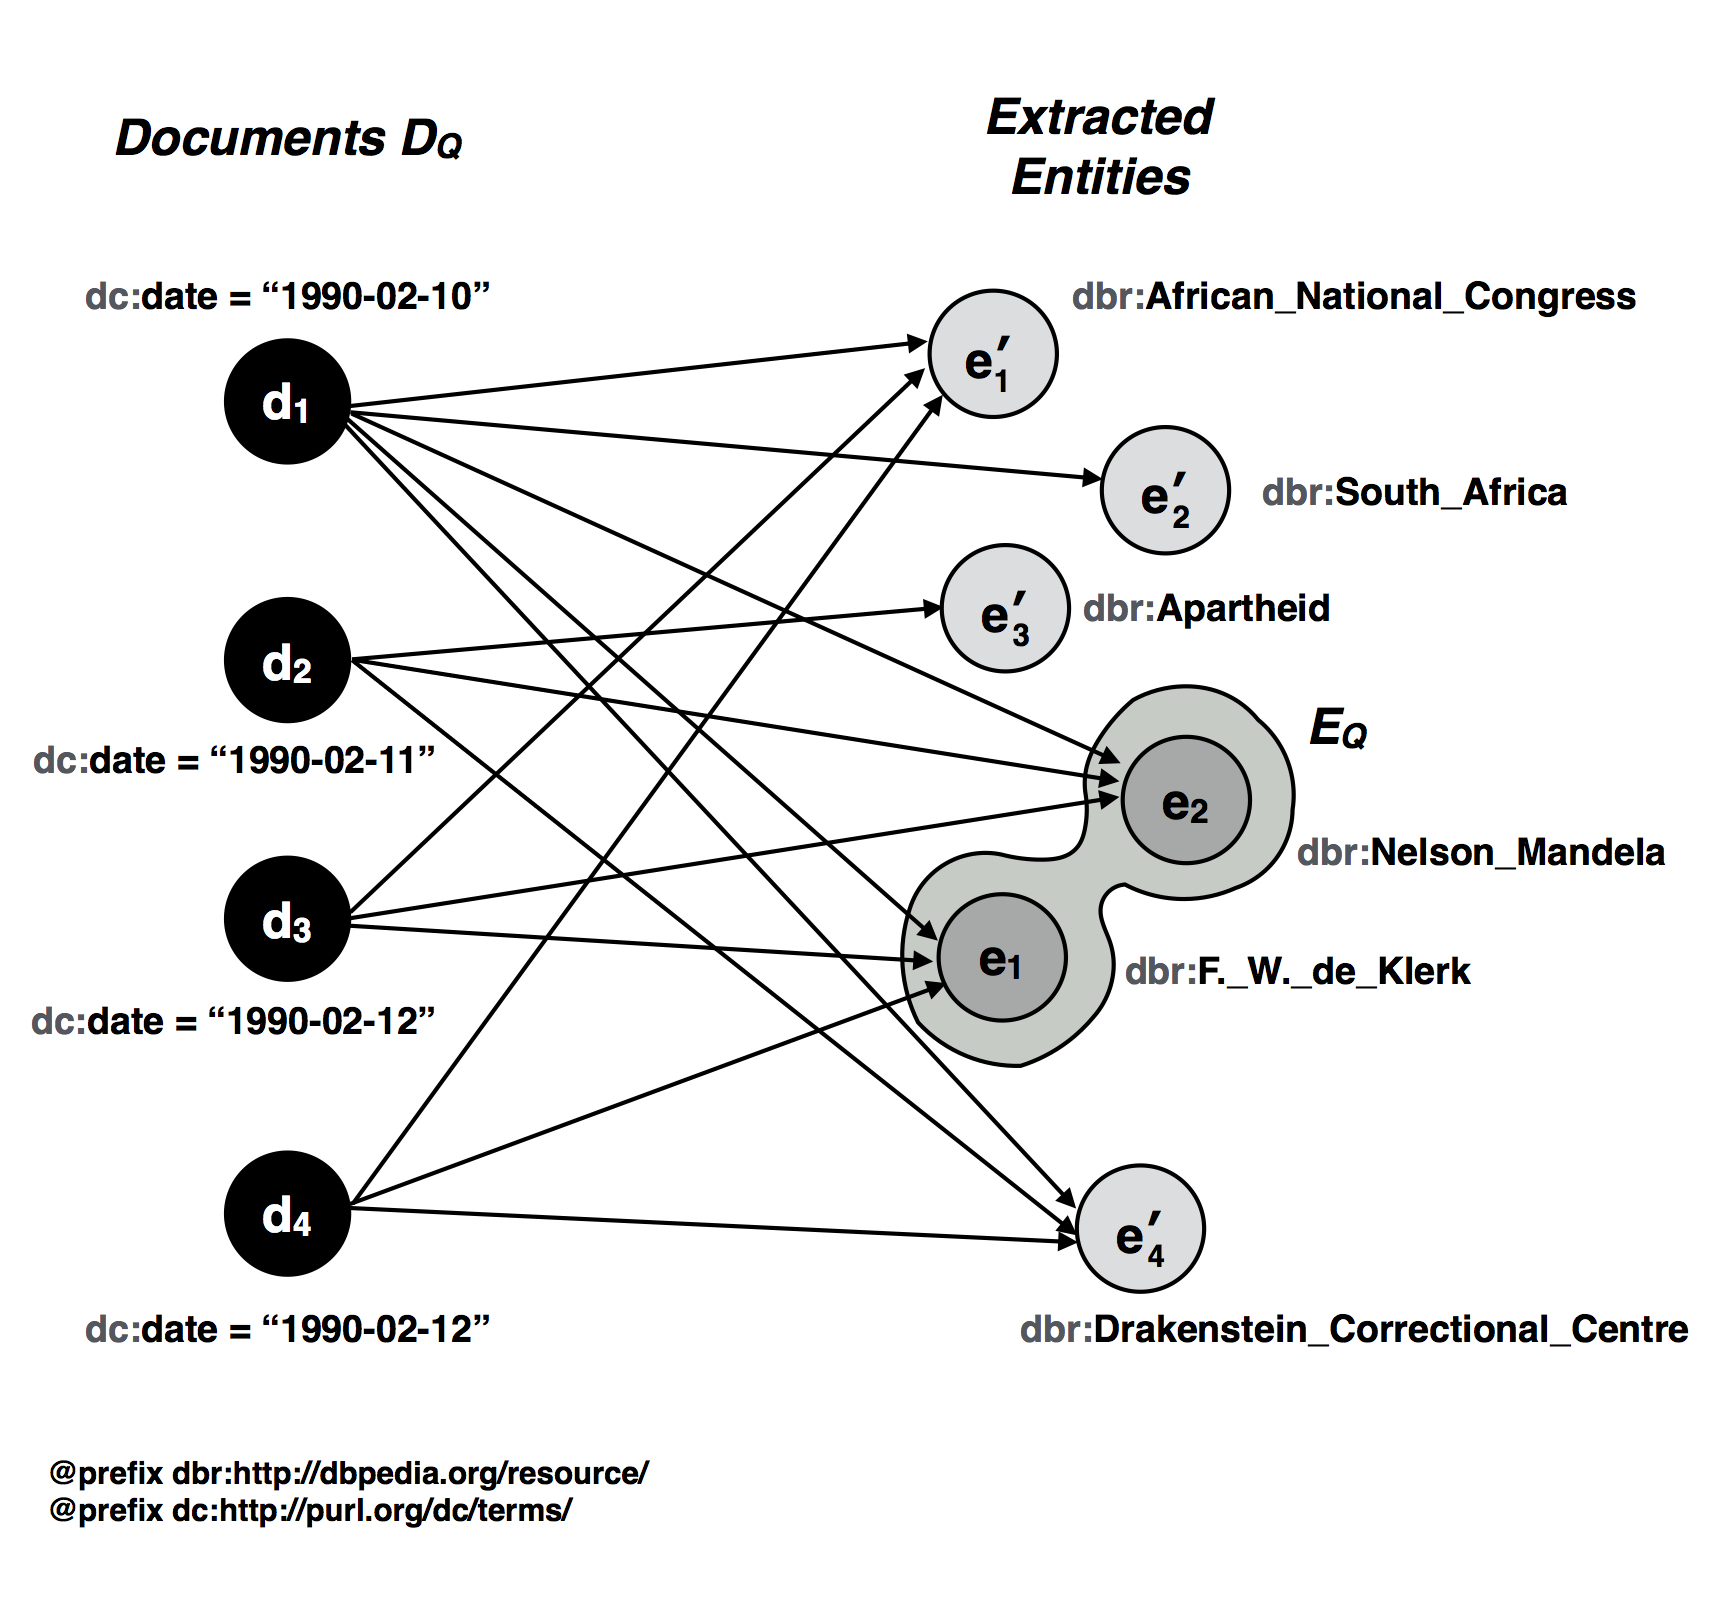
\includegraphics[width=0.8\textwidth]{revised_graph}
\end{mdframed}
    \caption{An example graph for the query {\em Nelson Mandela} {\tt OR}
                    {\em Frederik Willem de Klerk}}
    \label{fig:revised_graph}
\end{figure}
%=====}

\comment{======

When a query input is given by the user, a we define a graph $G = (V, E)$ in which the
node set $V$ consist of the documents obtained as results
of the SPARQL query $d$ such that
$d \in D_Q$, entities extracted from these documents $e'$ and the entities of interest $e, e \in E_Q$.
The edge set E consists of edges that are created between: a) every document node,
b) a document node to an entity of interest node if the document contains the
entity of interest,
c) a document node to an extracted entity node if the entity finds
a mention in the document node,
d) an entity of interest node to an extracted entity node
if they both are mentioned together in at least one result document and
denoted by $edge(e, e')$, and
e) an extracted entity node $e'$ to another extracted entity node $e''$ if both are
co-mentioned in at least one result document and denoted by $edge(e',e'')$.
In the case of {\tt AND} Semantics, there would be edges between every document and all
entities of interest nodes and an entity of interest node and all extracted entity nodes
since all the result documents will contain a mention of all the entities of interest.

Figure \ref{fig:sample_graph} shows an example of a small graph for the query {\em
Nelson Mandela} {\tt OR} {\em Frederik Willem de Klerk} for the time period 10-12
February 1990 along with outgoing edges from both entities of interest.

\begin{figure}[ht]
\begin{mdframed}
    \centering
    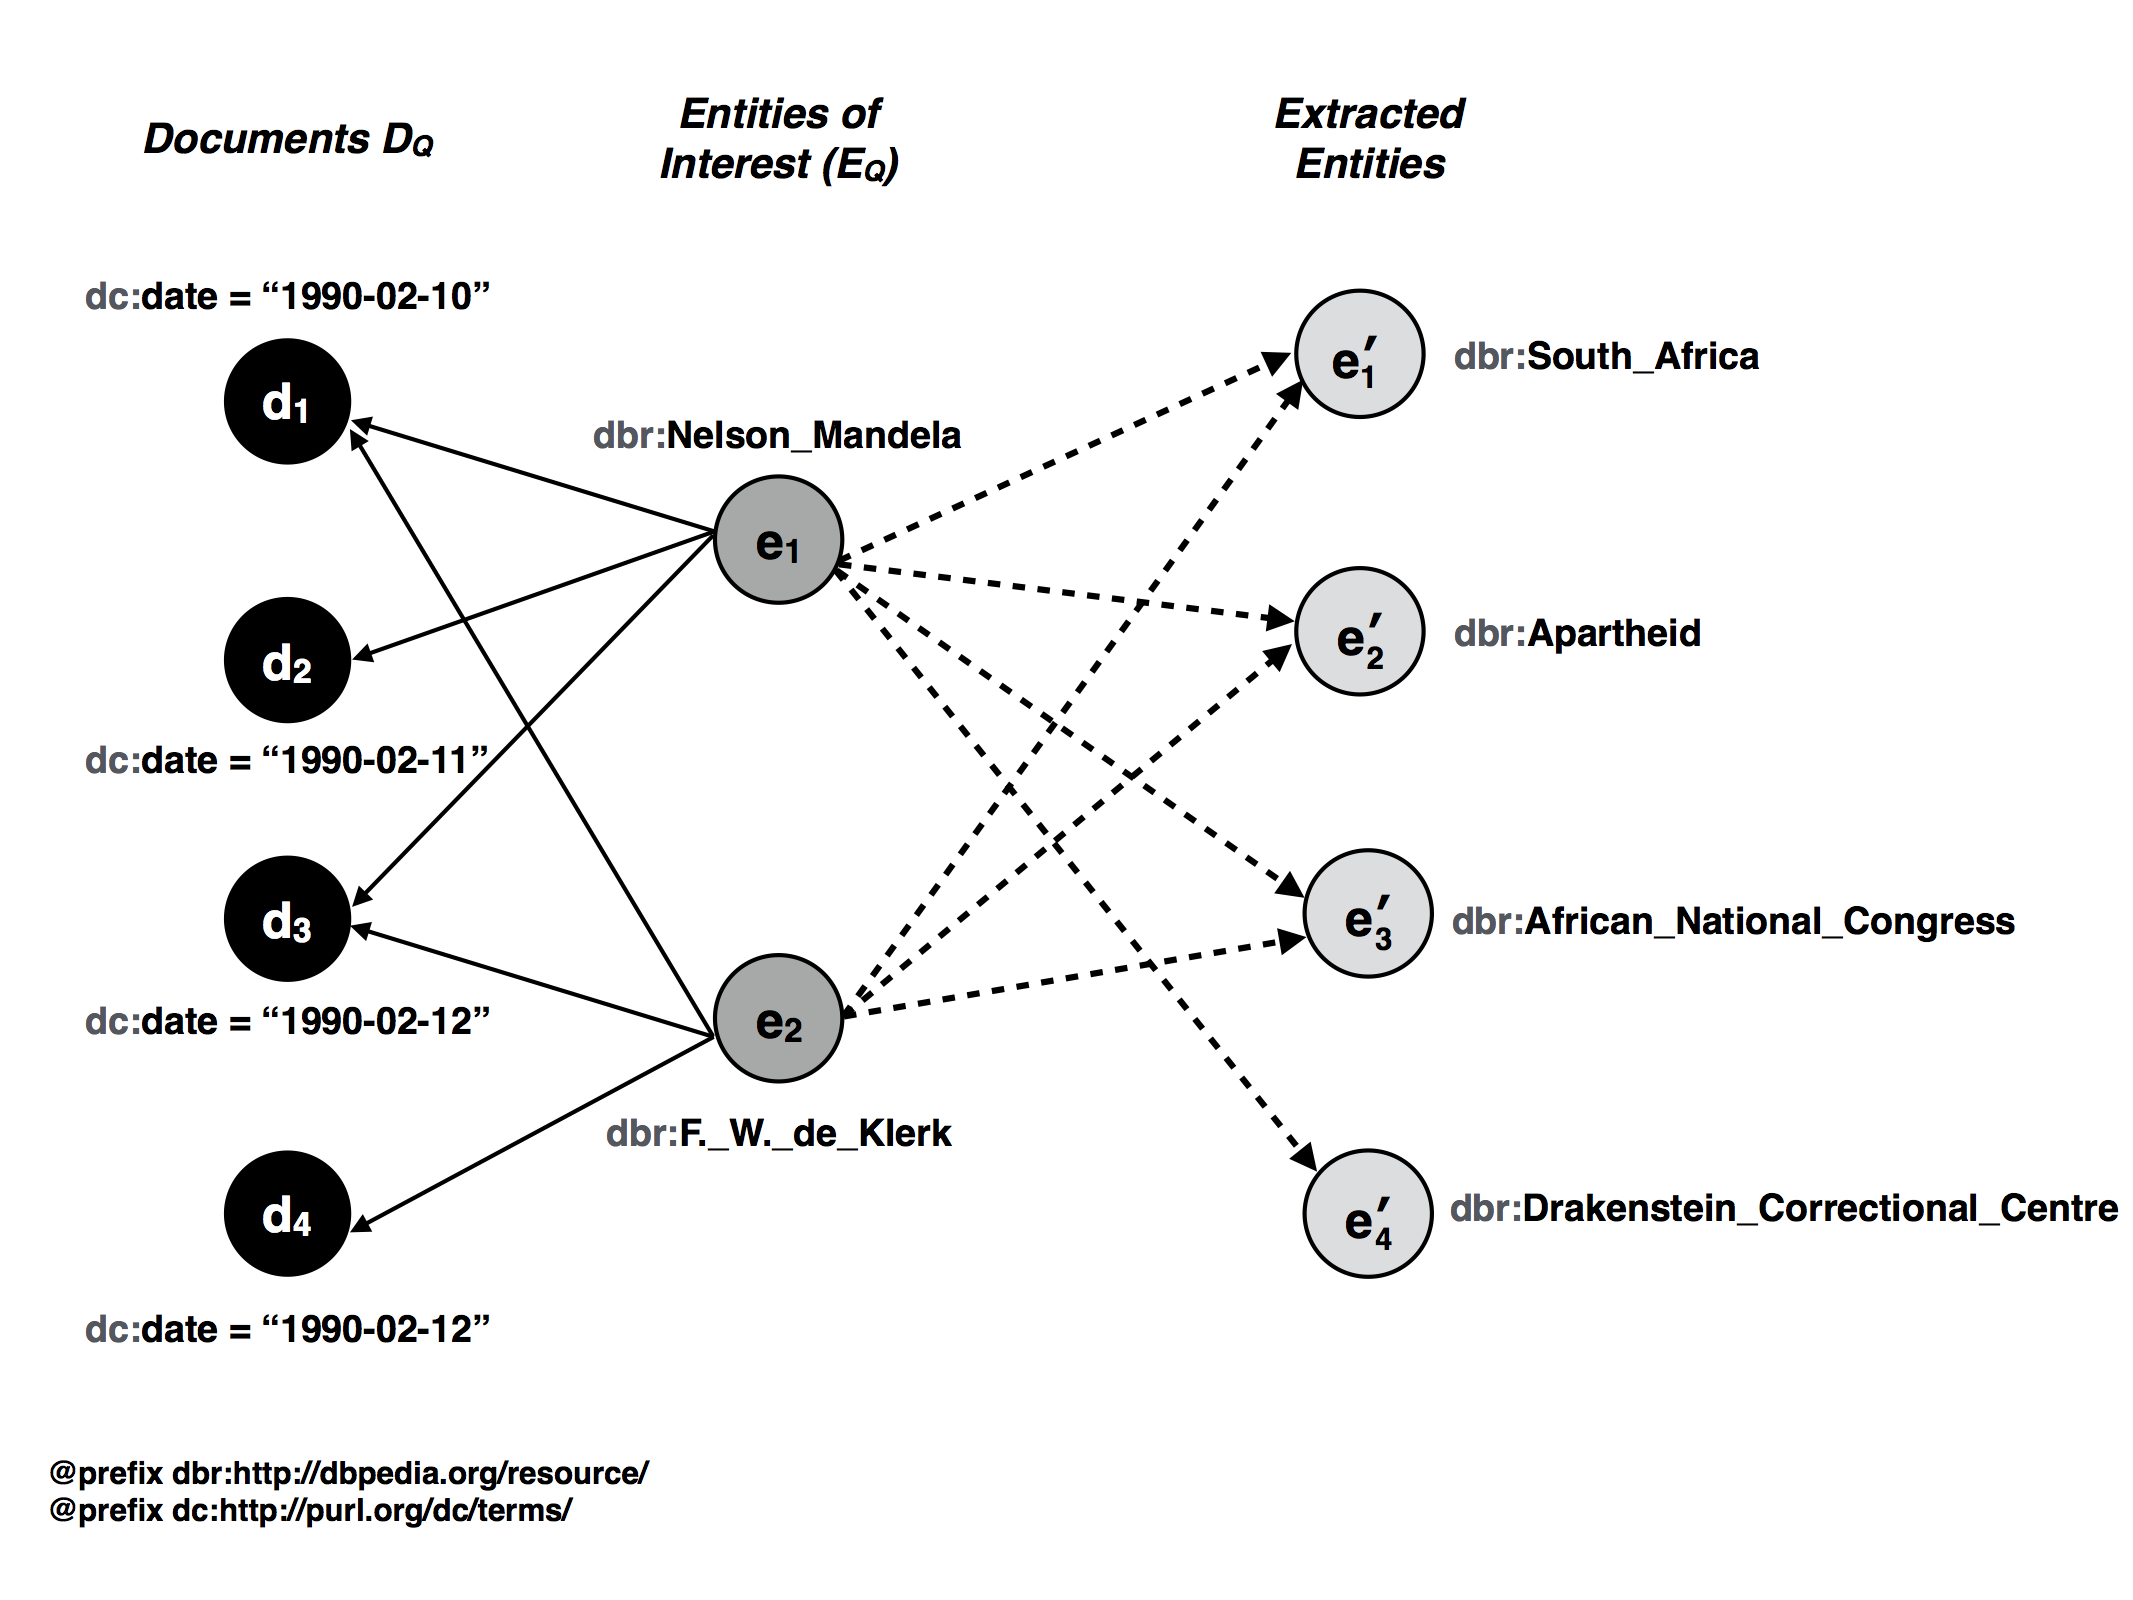
\includegraphics[width=0.95\textwidth]{sample_graph}
\end{mdframed}
    \caption{An example graph for the query {\em Nelson Mandela} {\tt OR}
                    {\em Frederik Willem de Klerk}}
    \label{fig:sample_graph}
\end{figure}

=====}

\subsection*{Creating a Transition Graph}

We create a transition graph $G' = (V', E')$ from $G$ where $V' = V$ and $E'$ contains
all edges in $E$ with an edge in the opposite direction for
each edge in E which has as one of the endpoints a document node,
that is, for each $edge(d, e) \in E$ we create $edge(e, d)$.
This is based on the notion that if a document  {\em contains} an
extracted entity,
then the extracted entity is also {\em contained} in the
document.

\comment{=======
We create a transition graph $G' = (V', E')$ from $G$ where $V' = V$ and $E'$ contains
all edges in $E$ with an edge in the opposite direction (if not already existing) for
each edge in E, that is, if $\nexists edge(e', e)$ and $edge(e, e')$ then we create
$edge(e', e)$.
This is based on the notion that if a document  {\em contains} an
extracted entity or an entity of interest,
then the extracted entity or the entity of interest is also {\em contained} in the
document. Similarly, if the entity of interest / an extracted entity
and another extracted entity are co-mentioned
together in at least a document, then it makes sense to have edges in both directions.
=====}

\subsection*{Describing Random Surfer behaviour}

Consider now a Random Surfer beginning at a node in this transition graph and
moving to other nodes.
In this scenario, the surfer can lie at either document nodes or
the extracted entity nodes or the entity of interest nodes.

\vspace{2mm}\noindent
If the random surfer begins at an entity node $e$ and $e \notin E_Q$,
then he can move to a document $d, d \in D_Q$ which contains the entity $e$.

\vspace{2mm}\noindent
It can also be the case that the surfer lies at a document node $d$.
In this case, he can transition to an entity $e$ existing/mentioned
in the document, i.e., $e \in ents(d)$.
Note that in this case $e$ could also be an entity of interest mentioned
in the document.

\vspace{2mm}\noindent
Lastly, the surfer can lie at an entity of interest $e'$.
In this case:
\begin{compactitem}
\item[(i)] With probability $p_1$ he moves to a document $d$, $d \in D_Q$, $e' \in ents(d)$.
\item[(ii)] With probability 1-$p_1$ he moves to an extracted entity $e$ which is co-mentioned
together with $e'$ in at least one returned document $d$, $d \in D_Q$.
\end{compactitem}

\comment{=====
Consider now a Random Surfer beginning at a node in this transition graph and
moving to other nodes. In this scenario, the surfer can lie at either document nodes,
extracted entity nodes or the entities of interest nodes.
If the random surfer begins at an entity of interest node $e$, then:
\begin{compactitem}
\item[(i)]  With probability $p_1$ he moves to a document $d, d \in D_Q$.
\item[(ii)] With probability 1-$p_1$ he moves to an extracted entity
$e'$ where $e' \in ents(d) \setminus E_Q$ and $d \in D_Q$.
\end{compactitem}

\vspace{2mm}\noindent
If the surfer is at a document $d$ and $d \in D_Q$, he moves:
\begin{compactitem}
\item[(i)]   With probability $p_2$ to another document $d', d' \in D_Q$.
\item[(ii)]  With probability $p_3$ to an entity of interest $e$.
\item[(iii)] With probability $1-p_2-p_3$ to an extracted entity
             $e', e' \in ents(d) \setminus E_Q $
\end{compactitem}

\vspace{2mm}\noindent
Lastly, the surfer can lie at an extracted entity $e'$.
In this case he can transition:
\begin{compactitem}
\item[(i)]   With probability $p_4$ to a document $d$ from which it was extracted,
             i.e., $d \in docs(e') \cap D_Q $.
\item[(ii)]  With probability $p_5$ to an entity of interest $e$.
\item[(iii)] With probability $1-p_4-p_5$ to another extracted entity $e''$.
\end{compactitem}

Figure \ref{fig:markov_chain} shows the Markov chain corresponding to this behaviour of
the Random Surfer.

\begin{figure}[ht]
\begin{mdframed}
    \centering
    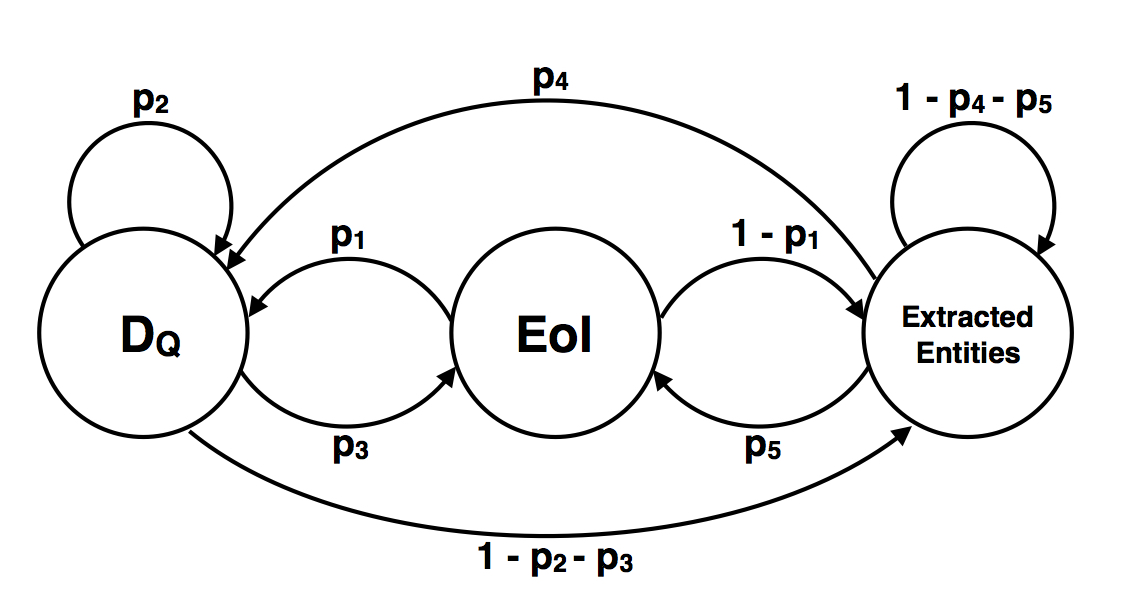
\includegraphics[width=0.5\textwidth]{markov_chain}
\end{mdframed}
    \caption{Markov chain showing Random Surfer behaviour}
    \label{fig:markov_chain}
\end{figure}
======}

\subsection*{Assigning edge weights}
The assignment of edge weights needs to be done keeping in mind that the
transition probabilities for a surfer from any node must sum up to 1, that is,
the weights of all the outgoing edges must sum to 1.
We describe weight assignment for each of the cases for nodes the random surfer can lie
at and all possible transitions it can make from this node.
As described above, the random surfer can only make three types of transitions and
in these types we assign edge weights as follows:

\vspace{2mm}\noindent
{\bf Case 1:} The surfer lies at an entity $e$, $e \notin E_Q$ and he moves to
a document $d \in D_Q$, i.e., the movement is along the edge $n \rightarrow n'$, where
$n=e$, and $n'=d, d \in D_Q$.

The weight of the edge ($n \rightarrow n'$) in this case ($n=e, n'=d$) for
both {\tt AND} and {\tt OR} semantics can be defined as:
\begin{equation}
\begin{split}
\small
weight(e \rightarrow d) = \frac{count(e,d)}{\sum_{d' \in docs(e) \cap D_Q}(count(e,d')}
\end{split}
\end{equation}

\vspace{2mm}\noindent
The criteria for assigning weight in the first case is based upon the
notion that from an entity a surfer is more likely to move to a document
that mentions the entity many times. %and is published in important
%time periods.


\vspace{2mm}\noindent
{\bf Case 2:} The surfer is at a document $d$ and moves to an entity $e, e \in ents(d)$.
The surfer transitions along the edge ($n \rightarrow n'$) where $n=d$ and $n'=e$.
We perform the weight assignment in this case as follows:
\begin{equation}
\begin{split}
\small
weight(d \rightarrow e) = \frac{count(e, d)}{\sum_{e' \in ents(d)}(count(e',d))}
\end{split}
\end{equation}
This means that a surfer is more likely to move from a document node to an entity
that finds mention more number of times in the document than other entities.

\vspace{2mm}\noindent
{\bf Case 3a:} The walker is at a an entity of interest $e'$ and he moves to
a document $d \in D_Q$, i.e., it transitions along the edge $n \rightarrow n'$, where
$n=e', e' \in E_Q$ and $n'=d, d \in D_Q$.

The weight of the edge ($n \rightarrow n'$) in this case ($n=e', n'=d$) for
both {\tt AND} and {\tt OR} semantics can be defined as:
\begin{equation}
\begin{split}
\small
weight(e' \rightarrow d) = \frac{score^{f}(d,E_Q)*score^{t}(t_d)}{\sum_{d' \in docs(e') \cap D_Q}(score^{f}(d',E_Q)*score^{t}(t_d'))}
\end{split}
\end{equation}

\vspace{2mm}\noindent
{\bf Case 3b:} The walker lies at an entity of interest $e'$ and moves to
a extracted entity $e$, i.e., it transitions along the edge ($n \rightarrow n'$) where
($n=e', n'=e$). Considering relatedness, for both {\tt AND} and {\tt OR} Semantics
we use the following criteria for assigning weights to the edges:
\begin{equation}
\begin{split}
\small
weight(e' \rightarrow e) = \frac{score^{r}(e)}{\sum_{e'' \in edge(e', e'')}(score^{r}(e''))}
\end{split}
\end{equation}
Here, for {\tt AND} and {\tt OR} semantics, we make use of the formulae described for $score^{r}(e)$
in the previous section accordingly.

\vspace{2mm}\noindent
Taking into consideration the transition probabilities,
the weight from an entity of interest-node $e'$ to a connected node $n$ can be
generally defined as:
\begin{gather}
\small
weight(e' \rightarrow n) = \begin{cases}
    p_1 \cdot \frac{score^{f}(d,E_Q)*score^{t}(t_d)}{\sum_{d' \in docs(e') \cap D_Q}(score^{f}(d',E_Q)*score^{t}(t_d'))}\qquad
    n = d, d \in D_Q\\
    (1-p_1) \cdot \frac{score^{r}(e)}{\sum_{e'' \in edge(e', e'')}(score^{r}(e''))}\qquad n = e, e \notin E_Q
\end{cases}
\end{gather}


\vspace{2mm}\noindent
The criteria for assigning weight in the third case is based upon the
notion that from an entity of interest a surfer is more likely to move to a document
that mentions the entity of interest many times and is published in important
time periods (for EoI). It is also likely to move to an extracted entity that it
finds frequently co-mentioned in documents together with the entities of interest.


\comment{======

\vspace{2mm}\noindent
{\bf Case 1a:} The surfer lies at an entity of interest $e$ and he moves to
a document $d \in D_Q$, i.e., the movement is along the edge $n \rightarrow n'$, where
$n=e, e \in E_Q$ and $n'=d, d \in D_Q$.

The weight of the edge ($n \rightarrow n'$) in this case ($n=e, n'=d$) for
both {\tt AND} and {\tt OR} semantics can be defined as:
\begin{equation}
\begin{split}
\small
weight(e \rightarrow d) = \frac{ScoreD^{f,t}(d)}{\sum_{d' \in D_Q}(ScoreD^{f,t}(d'))}
\end{split}
\end{equation}

\vspace{2mm}\noindent
{\bf Case 1b:} The walker lies at an entity of interest $e$ and moves to
a extracted entity $e'$, i.e., it transitions along the edge ($n \rightarrow n'$) where
($n=e, n'=e'$). Considering relatedness, for both {\tt AND} and {\tt OR} Semantics
we use the following criteria for assigning weights to the edges:
\begin{equation}
\begin{split}
\small
weight(e \rightarrow e') = \frac{ScoreE(e')}{\sum_{\exists edge(e, e''), e'' \in ents(d) \setminus E_Q, d \in D_Q}(ScoreE(e''))}
\end{split}
\end{equation}

Taking into consideration the transition probabilities,
the weight from an entity-node e to a connected node $n$ can be
generally defined as:
\begin{gather}
\small
weight(e \rightarrow n) = \begin{cases}
    p_1 \cdot \frac{ScoreD^{f,t}(d)}{\sum_{d' \in D_Q}(ScoreD^{f,t}(d'))} \qquad
    n = d\\
    (1-p_1) \cdot \frac{ScoreE(e')}{\sum_{\exists edge(e, e''), e'' \in ents(d) \setminus E_Q, d \in D_Q}(ScoreE(e''))}
    \qquad n = e'
\end{cases}
\end{gather}


\vspace{2mm}\noindent
The criteria for assigning weight in the first case is based upon the
notion that from an entity of interest a surfer is more likely to move to a document
that mentions the entity of interest many times and is published in important
time periods (for EoI). It is also likely to move to an extracted entity that it
finds frequently co-mentioned in documents together with the entities of interest.

\vspace{2mm}\noindent
{\bf Case 2a:} The walker is at a document $d$ and moves to another document $d' \in D_Q$,
i.e., the walker moves along the edge $n \rightarrow n'$ where $n=d$ and $n'=d'$.
In this case, we use the following criterion for assigning weight to the edge:
\begin{equation}
\begin{split}
\small
weight(d \rightarrow d') = \frac{ScoreD^{c}(d')}{\sum_{d'' \in D_Q , d'' \neq d}(ScoreD^{c}(d''))}
\end{split}
\end{equation}

\vspace{2mm}\noindent
{\bf Case 2b:} The walker is at a document $d$ and moves to an entity of interest $e$,
i.e., the movement is along the edge ($n \rightarrow n'$) where $n=d$ and $n'=e$.
We perform the weight assignment in this case as follows:
\begin{equation}
\begin{split}
\small
weight(d \rightarrow e) = \frac{1}{|ents(d) \cap E_Q|}
\end{split}
\end{equation}
This means that we define that it is equiprobable for a surfer to move to any of the
entities of interest from a document containing the EoI. In case the document mentions
only one EoI, then weight becomes equal to 1.

\vspace{2mm}\noindent
{\bf Case 2c:} The walker is at a document $d$ and moves to an entity $e'$ extracted
from it, i.e., $e' \in ents(d) \setminus E_Q$.
The surfer transitions along the edge ($n \rightarrow n'$) where $n=d$ and $n'=e'$.
We perform the weight assignment in this case as follows:
\begin{equation}
\begin{split}
\small
weight(d \rightarrow e') = \frac{1}{|ents(d) \setminus E_Q|}
\end{split}
\end{equation}
This means that there is an equal probability for the surfer to move from a document
to any entity extracted from the document, the entity not being the entity of interest.

\vspace{2mm}\noindent
Like in the first case, in the second case as well, due to transition probabilities we
define the weight from an entity-node d to a connected node n as:
\begin{gather}
\small
weight(d \rightarrow n) = \begin{cases}
    p_2 \cdot \frac{ScoreD^{c}(d')}{\sum_{d'' \in D_Q , d'' \neq d}(ScoreD^{c}(d''))}
    \qquad n = d'\\
    p_3 \cdot \frac{1}{|ents(d) \cap E_Q|}
    \qquad n = e\\
    (1-p_2-p_3) \cdot \frac{1}{|ents(d) \setminus E_Q|} \qquad n = e', p_2+p_3 \leq 1
\end{cases}
\end{gather}

\vspace{2mm}\noindent
In the second case, we assign weight of an edge when moving to another document based
on the temporal closeness aspect.
The surfer can also move to an entity which he finds a mention in a document or back to
an entity of interest.

\vspace{2mm}\noindent
{\bf Case 3a:} The surfer lies at an extracted entity $e'$ and
moves to a document $d$ from which it was extracted, i.e., $d \in docs(e') \cap D_Q $.
It transits along the edge ($n \rightarrow n'$) where $n=e'$ and $n'=d'$.
We take into the number of occurrences of the extracted entity in the documents
and define the weight assignment as:
\begin{equation}
\begin{split}
\small
weight(e' \rightarrow d) = \frac{count(e', d)}{\sum_{d' \in docs(e') \cap D_Q}(count(e',d'))}
\end{split}
\end{equation}
The edge weight of an extracted entity to a document node is higher if the extracted
entity is mentioned more number of times in the document.

\vspace{2mm}\noindent
{\bf Case 3b:} The surfer is at an extracted entity $e'$ and
transitions to an entity of interest $e$, i.e., it travels along the edge
($n \rightarrow n'$) where $n=e'$ and $n'=e$.
We define the weight assignment as:
\begin{equation}
\begin{split}
\small
weight(e' \rightarrow e) = \frac{1}{|edge(e', e'')|} \qquad e'' \in E_Q
\end{split}
\end{equation}
This equation translates as: there is equal probability for a
walker to move from a extracted entity $e'$ to any of the entities of interest
connected to it by an edge. In case the related entity is connected to only one
entity of interest, the weight of the edge becomes 1.


\vspace{2mm}\noindent
{\bf Case 3c:} The surfer transitions to another extracted entity $e''$ from an
extracted entity $e'$. It moves along the edge
($n \rightarrow n'$) where $n=e'$ and $n'=e''$.
We define the weight assignment as:
\begin{equation}
\begin{split}
\small
weight(e' \rightarrow e'') = \frac{1}{|edge(e', e''')|} \qquad \exists d \enskip
s.t. \enskip d \in docs(e') \cap docs(e''')
\end{split}
\end{equation}
We assign an equal weight to any entity co-mentioned together with an extracted entity
in at least a document.

To make sum of  weights of all outgoing links as 1, we define the weight from an
extracted entity-node e' to a connected node n as:
\begin{gather}
\small
weight(e' \rightarrow n) = \begin{cases}
    p_4 \cdot \frac{count(e', d)}{\sum_{d' \in docs(e') \cap D_Q}(count(e',d'))} \qquad
    n = d'\\
    p_5 \cdot \frac{1}{|edge(e', e'')|} \qquad n = e, e'' \in E_Q \\
    (1-p_4-p_5) \cdot  \frac{1}{|edge(e', e''')|} \qquad \exists d \enskip s.t. \enskip
    d \in docs(e') \cap docs(e'''), n = e'',p_4 + p_5 \leq 1
\end{cases}
\end{gather}

======}

\subsection*{Analyzing the Transition Graph}
For a node $n$, let $in(n)$ be the set of nodes with in-links to n.
We define the {\em PageRank-like} value $r(n)$ as:
\begin{equation}
\begin{split}
\small
r(n) = d \cdot Jump(n) + (1-d) \cdot \sum_{n' \in in(n)}{(weight(n \rightarrow n') \cdot r(n'))}
\end{split}
\end{equation}
In this equation d is the {\em decay factor} or in other words,
the probability for the surfer to perform a random jump and
with probability {\em Jump(n)} the surfer jumps to node n.
The probability of the walker to transit to node $n$ from a connected
node $n'$ is given by $weight(n \rightarrow n')$.
Sufficient number of iterations should be performed so as to
allow the algorithm to converge.
\new{In our experiments we fixed the number of iterations to 30.}

\subsection*{Fixing Random Jumps and Tuning}
Initially, we start by assigning a PageRank score only to entities of interest. 
Each entity of interest gets assigned a score equal to 1 
divided by the number of entities of interest and all other nodes a score of 0.  
We fix random jumps such that the surfer can perform random jumps only
to entity of interest nodes.
Additionally, when performing a random jump, a surfer only jumps 
equiprobably to any of the entity of interest nodes.
We test the algorithm for decay factor values of 0.0, 0.2, 0.5 and 0.8.
A value of 0 for the decay factor means that there is no possibility
for the surfer to perform a random jump and a value of 1 translates
to the surfer only perform jumps from one entity of interest to another
entity of interest.

We also vary the $p_1$ values to see which combination of edge weights leads to
the best ranking.
A higher $p_1$ value implies that the edge weights for edges between
entity of interest nodes and document nodes increases which might lead to the
surfer moving to a highly relevant document from an entity of interest.
On the other hand, a lower $p_1$ values leads to increase in the edge weight
between entity of interest nodes and extracted entity nodes
which might be beneficial
as the surfer would have greater chance to move to a highly
related entity node from the
entity of interest node and from there it can further transition to
a highly relevant document node.
The algorithm is tested for different values of $p_1$ to see which
combination leads to the best ranking.
A value of 0 for $p_1$ implies that we the surfer can reach the
document nodes from the entity of interest
nodes only through the entity nodes thus assigning more importance
to highly related entities.
Conversely, a $p_1$ value of 1 would mean that only direct transition is possible from
entity of interest node to a document node making documents
mentioning the entity of interest many times
and published in important time periods more important.